
\documentclass{article}
\usepackage{amsmath, amssymb, graphicx, times}
\usepackage[margin=1in]{geometry}
\usepackage{natbib}
\usepackage{hyperref}
\title{Viewing Gradient Flow as Reverse Diffusion: A Thermodynamic and Probabilistic Perspective}
\author{Anonymous Author(s)}
\date{}

\begin{document}
\maketitle

\begin{abstract}
Gradient-based optimization lies at the core of modern machine learning. In this paper, we provide a new perspective on gradient descent dynamics by interpreting them as reverse-time probability flows akin to those used in diffusion-based generative models. Drawing connections between Wasserstein gradient flows, Fokker-Planck equations, and score-based diffusion models, we propose that gradient descent trajectories in parameter space can be understood as the deterministic reversal of an underlying stochastic diffusion process. This thermodynamic viewpoint not only unifies disparate concepts in optimization and probabilistic modeling but also offers a blueprint for novel algorithmic designs rooted in stochastic thermodynamics.
\end{abstract}

\section{Introduction}
Einstein's theory of Brownian motion inspired the modern theory of stochastic processes. In parallel, diffusion-based generative models transform data distributions into noise via SDEs and reverse the process for generation. We explore the hypothesis that gradient descent dynamics are reverse-time ODEs of some underlying forward diffusion process.

\section{Background}
\subsection{Fokker-Planck and Brownian Motion}
The diffusion of a particle is governed by:
\[
\partial_t \rho(x,t) = D \nabla^2 \rho(x,t)
\]
A general SDE:
\[
dx = f(x,t)dt + g(t) dW_t
\]
has a density governed by:
\[
\partial_t \rho = -\nabla \cdot (f \rho) + \frac{1}{2} \nabla^2(g^2 \rho)
\]

\subsection{Diffusion Models in Machine Learning}
Score-based models define forward SDEs and reverse-time SDEs:
\[
dx = [f(x,t) - g(t)^2 \nabla_x \log p_t(x)] dt
\]
The deterministic variant is known as the probability flow ODE.

\section{Gradient Descent as Probability Flow}
The ODE of gradient descent:
\[
\frac{d\theta}{dt} = -\nabla_\theta L(\theta)
\]
is equivalent in form to a probability flow ODE under a parameter distribution $\rho(\theta,t)$:
\[
\partial_t \rho + \nabla_\theta \cdot (\rho \nabla_\theta L) = 0
\]

\section{Constructing Forward SDEs}
We propose a forward SDE whose reverse-time flow resembles gradient descent. This formulation connects optimization with generative diffusion models.

\section{Toy Experiment}
We simulate a toy 2D quadratic loss and its diffusion process. Figure~\ref{fig:trajectory} compares gradient flow and reverse diffusion.

\begin{figure}[h]
\centering
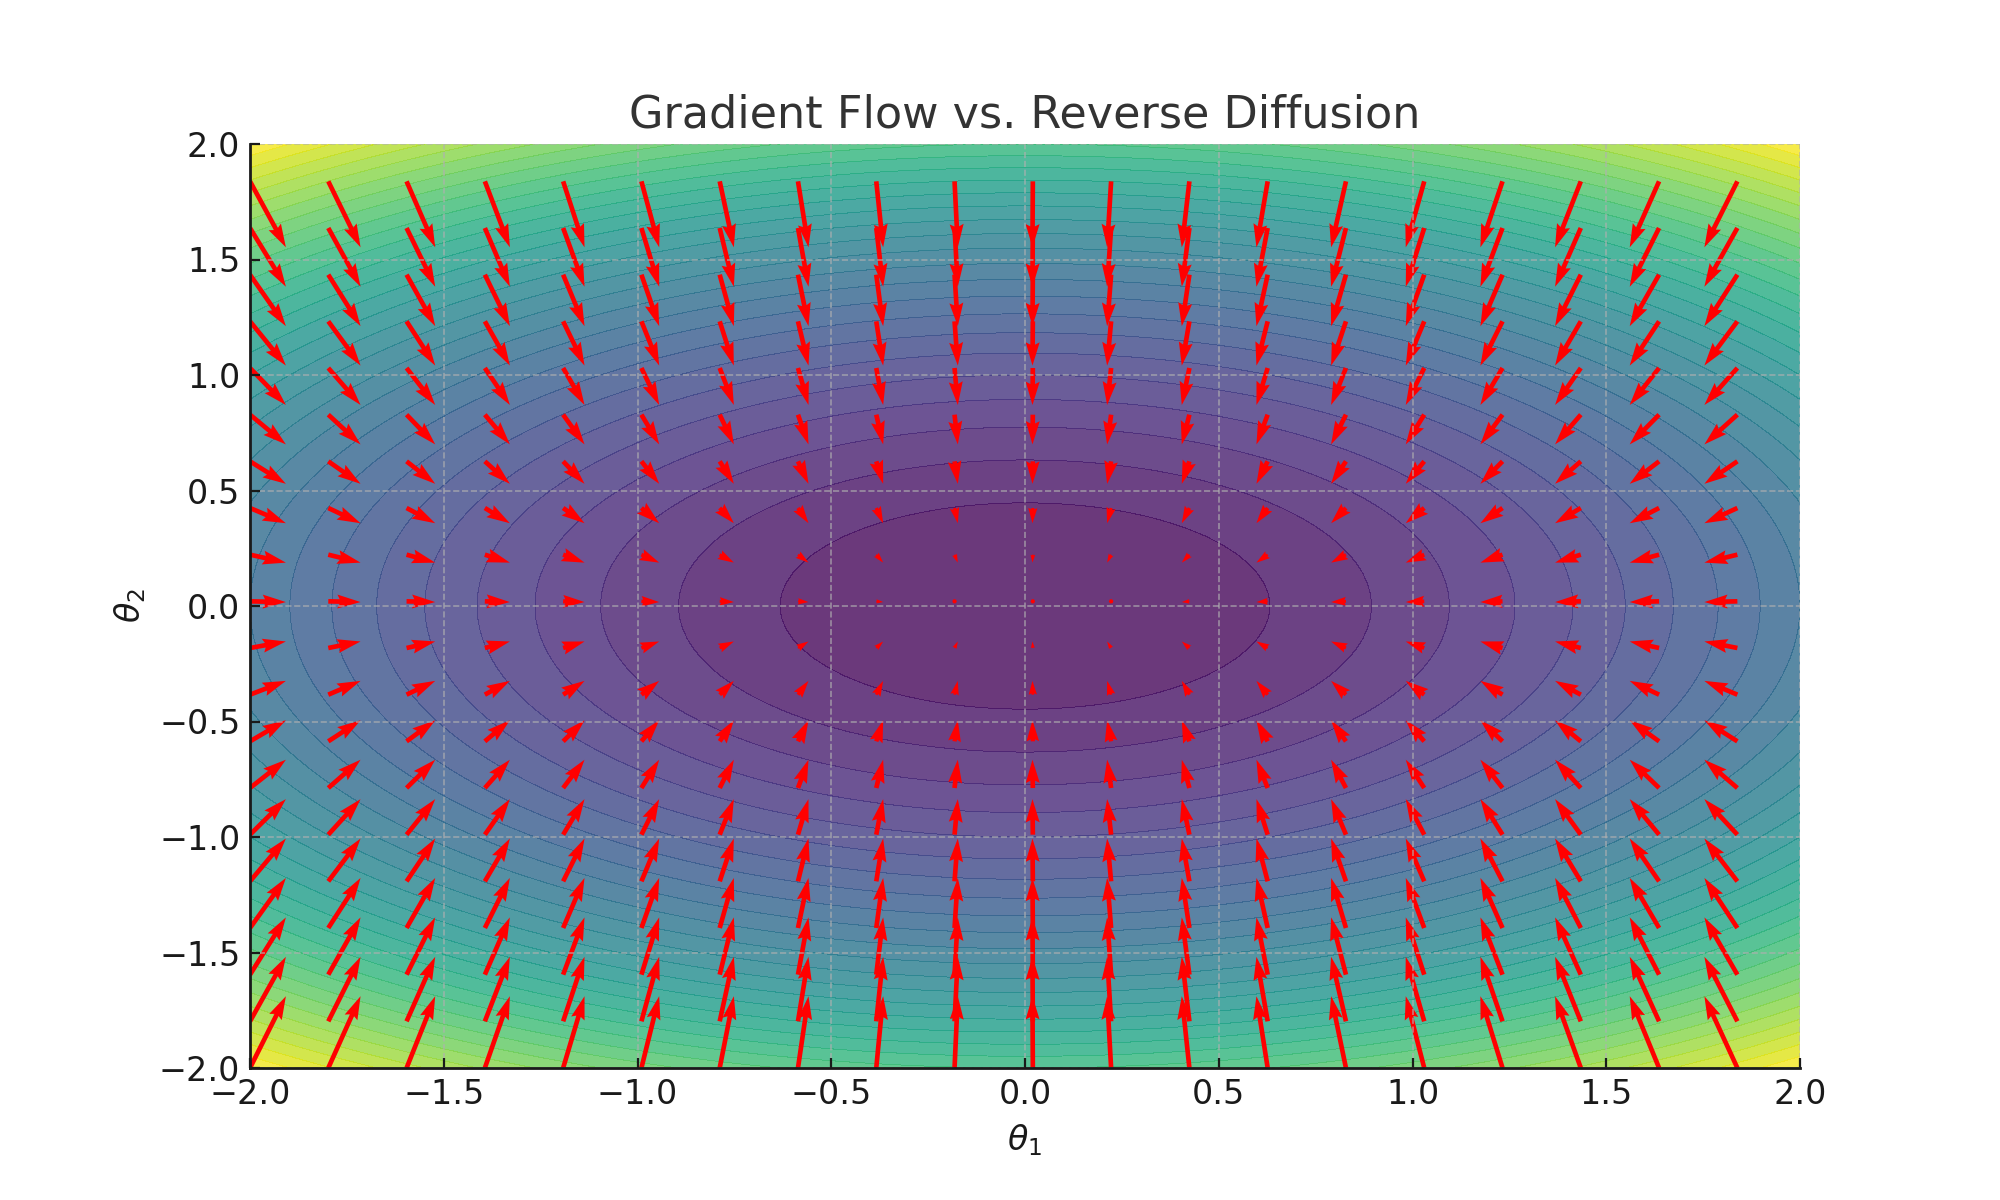
\includegraphics[width=0.65\textwidth]{figures/trajectory.png}
\caption{Gradient descent trajectory vs. reverse diffusion flow on 2D loss surface.}
\label{fig:trajectory}
\end{figure}

\section{Conclusion}
Gradient descent can be viewed as a reverse-time probability flow ODE. This perspective offers a theoretical bridge between optimization and diffusion-based generative modeling.

\bibliographystyle{plain}
\bibliography{refs}

\end{document}
